% !TEX program = lualatex 

\documentclass[9pt]{beamer}

\usetheme{metropolis}
\usepackage{bookmark}
\usepackage{xcolor-solarized}

\setbeamercolor{normal text}{%
  fg=solarized-base02,
  bg=solarized-base3!20!white
}
\setbeamercolor{alerted text}{%
  fg=solarized-red
}
\setbeamercolor{example text}{%
  fg=solarized-green
}
\setbeamercolor{frametitle}{%
    fg=solarized-blue!70!black,
    bg=solarized-base2
}

\setbeamerfont{title}{series=\bfseries,parent=structure}
\setbeamerfont{frametitle}{series=\bfseries,parent=structure}
\renewcommand{\footnotesize}{\scriptsize}
% sort
\newcommand{\issortedany}{\term{in-image}}
\newcommand{\issorted}{\issortedany_s}
\newcommand{\isheadleast}{\term{image-respects-pair}}
\newcommand{\istailsort}{\term{image-can-induct}}
\newcommand{\setord}{\term{Ord}}
\newcommand{\Ord}{\term{Ord}}
\newcommand{\setmtol}{\term{M2L}}
\newcommand{\setsort}{\term{Sort}}
\newcommand{\Sort}{\term{Sort}}
\newcommand{\otof}{\term{o2f}}
% constructions
\newcommand{\List}{\term{List}}
\newcommand{\Array}{\term{Array}}
\newcommand{\PList}{\term{PList}}
\newcommand{\SList}{\term{SList}}
\newcommand{\Bag}{\term{Bag}}
\newcommand{\Perm}{\term{Perm}}


\usecolortheme{orchid}

\usepackage{hott}
\usepackage{mathtools}
\usepackage{macros}
\usepackage[final]{microtype}

\usepackage{mathpartir}
\usepackage{worldflags}
\usepackage{stmaryrd}
\usepackage{lipsum}
\usepackage{adjustbox}
\usepackage{amsmath}
\usepackage{amssymb}
\usepackage{geometry}
\usepackage{mathrsfs}
\usepackage{braket}
\usepackage{quiver}
\usepackage{mathtools}
\usepackage{commath}
\usepackage{xparse}
\usepackage{array}
\usepackage{subcaption} %side by side diagrams
\usepackage{floatrow}
\usepackage{tikz}
\usepackage{tikz-cd}
\usetikzlibrary{babel}% added

% bibliography
\usepackage[style=authortitle,backend=biber]{biblatex}
\addbibresource{../../symmetries.bib}

% fancy boxes
\usepackage[most]{tcolorbox}

\newtcolorbox{qblock}[1][Question]{
  colback=white,
  colframe=solarized-orange,
  colbacktitle=white!90!structure.fg,
  coltitle=black,
  fonttitle=\itshape,
  title={#1},
  enhanced,
  attach boxed title to top left={yshift=-0.1cm, xshift=0.5em}
}
\newtcolorbox{dblock}[1][Definition]{
  colback=white,
  colframe=solarized-violet,
  colbacktitle=white!90!structure.fg,
  coltitle=black,
  fonttitle=\itshape,
  title={#1},
  enhanced,
  attach boxed title to top left={yshift=-0.1cm, xshift=0.5em}
}

\newtcolorbox{pblock}[1][Proposition]{
  colback=white,
  colframe=solarized-blue,
  colbacktitle=white!90!structure.fg,
  coltitle=black,
  fonttitle=\itshape,
  title={#1},
  enhanced,
  attach boxed title to top left={yshift=-0.1cm, xshift=0.5em}
}

\newtcolorbox{tblock}[1][Theorem]{
  colback=white,
  colframe=solarized-green,
  colbacktitle=white!90!structure.fg,
  coltitle=black,
  fonttitle=\itshape,
  title={#1},
  enhanced,
  attach boxed title to top left={yshift=-0.1cm, xshift=0.5em}
}

\usepackage{tikz}
\usetikzlibrary{cd}
\usetikzlibrary{fit}

\usepackage{fontspec}
\setmonofont{Iosevka}[
    Path=./Iosevka/,
    Extension = .ttf,
    UprightFont=*-Regular,
    BoldFont=*-Bold,
    ItalicFont=*-Italic,
    BoldItalicFont=*-BoldItalic
]

%Information to be included in the title page:
\title{Order from sorting with universal algebra}
\author[shortname]{
  Wind Wong \inst{1}
  \and Vikraman Choudhury \inst{2}
  \and Simon J. Gay \inst{1}
}
\institute[shortinst]{\inst{1} University of Glasgow \and %
                      \inst{2} Universit\`{a} di Bologna and OLAS Team, INRIA}
\date{February 14, 2024}

\begin{document}

\frame{\titlepage}

\begin{frame}
  \frametitle{Introduction}

  
  Consider a puzzle about sorting,
inspired by Dijkstra's Dutch National Flag problem~\footcite{dijkstraDisciplineProgramming1997}.
Suppose there are balls of three colors,
corresponding to the colors of the Dutch flag: red, white, and blue.
\[
  \{
  \tikz[anchor=base, baseline]{%
    \foreach \x/\color in {1/red,2/white,3/blue} {
        \node[circle,draw,fill=\color,line width=1pt] at (\x,0) {\phantom{\tiny\x}};
        \ifthenelse{\NOT 1 = \x}{\node at ({\x-0.5},0) {,};}{}
      }
  }
  \}
\]
  Given an \alert{unordered list} of such balls, how many ways can you \alert{sort} them into the Dutch flag?
\[
  \{
      \tikz[anchor=base, baseline]{%
        \foreach \x/\color in {1/red,2/red,3/blue,4/white,5/blue,6/red,7/white,8/blue} {
            \node[circle,draw,fill=\color,line width=1pt] at (\x,0) {\phantom{\tiny\x}};
            \ifthenelse{\NOT 1 = \x}{\node at ({\x-0.5},0) {,};}{}
          }
      }
    \}
\]
  Obviously there is \alert{only one} way, which is given by the order
  \alert{$\term{red} < \term{white} < \term{blue}$}.
\[
  [
      \tikz[anchor=base, baseline]{%
        \foreach \x/\color in {1/red,2/red,3/red,4/white,5/white,6/blue,7/blue,8/blue} {
            \node[circle,draw,fill=\color,line width=1pt] at (\x,0) {\phantom{\tiny\x}};
            \ifthenelse{\NOT 1 = \x}{\node at ({\x-0.5},0) {,};}{}
          }
      }
    ]
\]

\end{frame}

\begin{frame}{Introduction}

  What if we are avid enjoyers of vexillology who also want to consider other flags?

We might ask: how many ways can we sort our bag of balls?

We know that there are only $3! = 6$ permutations of
  $\{\term{red}, \term{white}, \term{blue}\}$, so there are only \alert{6 possible orderings} we can define.
  \footnote{I have no allegiance to any of the countries presented by the flags, hypothetical or otherwise -- this is purely combinatorics!}
\vspace{0.5em}
\begin{center}
    \foreach \colorA/\colorB/\colorC in {red/white/blue, red/blue/white, white/red/blue, white/blue/red, blue/red/white, blue/white/red}{
    
\begin{tikzpicture}[scale=0.5]
    \begin{flagdescription}{3/4}
    \hstripesIII{\colorA}{\colorB}{\colorC}
    \framecode{}
    \end{flagdescription}
    \end{tikzpicture}
    }
\end{center}

  We claim because there are \alert{exactly 6 orderings},
  we can only define \alert{6 \textit{correct} sorting functions}.

\vspace{0.5em}

\end{frame}

\begin{frame}{Introduction}

\only<1>{
More formally,
  \begin{itemize}
    \item Let $A = \{\term{red}, \term{white}, \term{blue}\}$
    \item Let $\setord(A)$ be the \alert{set of orderings} on $A$
    \item Let $\setmtol(A)$  be the \alert{set of functions} $\term{UnorderedList}(A) \to \List(A)$
  \end{itemize}

There is a function $\otof : \setord(A) \to \setsort(A)$ that maps orderings to
  some \alert{subset} $\setsort(A) \subset \setmtol(A)$ which we call \alert{"sort functions"}:
}

\begin{center}
    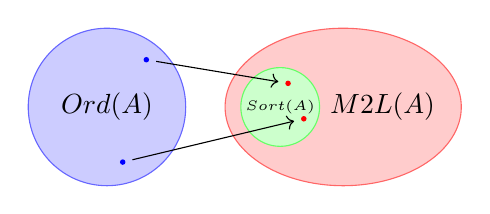
\begin{tikzpicture}
        % draw the sets
        \filldraw[fill=blue!20, draw=blue!60] (-1.5,0) circle (1cm);
        \filldraw[fill=red!20, draw=red!60] (1.5,0) ellipse (1.5cm and 1cm);
        \filldraw[fill=green!20, draw=green!60] (0.7,0) circle (0.5cm);
    
        % the texts
        \node at (-1.5,0) {$\Ord(A)$};
        \node at (0.7, 0) {\tiny$\Sort(A)$};
        \node at (2,0) {$\setmtol(A)$};

    
        % the points in the sets (here I just create nodes to use them later on to position
        % the circles and the arrows
        \node (x1) at (-1,0.6) {};
        \node (x2) at (-1.3,-0.7) {};
        \node (y1) at (0.8,0.3) {};
        \node (y2) at (1,-0.15) {};
    
        % position the elements in the sets (at the nodes we just created)
        \fill[blue] (x1) circle (1pt);
        \fill[blue] (x2) circle (1pt);
        \fill[red] (y1) circle (1pt);
        \fill[red] (y2) circle (1pt);
    
        % draw the arrows
        \draw[->] (x1) -- (y1);
        \draw[->] (x2) -- (y2);
    \end{tikzpicture}
\end{center}

\only<2>{
  This \textit{seems} trivial to prove.

  Construct $\otof(r)$ by parameterizing any sorting algorithm
  by the order relation $r$ and we are done!

  But\dots

  We want to show that there are \alert{exactly 6 sorting functions} because
  there are \alert{exactly 6 orderings}.

  $\otof(r)$ should be an \alert{isomorphism} from $\setord(A)$ to $\setsort(A)$.

  What is the \alert{inverse} of $\otof(r)$?
}

\end{frame}

\begin{frame}{Plan}
  To study this we need to execute the following plan:
  \vspace{2em}

  \only<1>{
    1. Formalize what \alert{$\term{UnorderedList}(A)$} and \alert{$\List(A)$} are.
      \begin{itemize}
        \item  Create a \alert{universal algebra framework} which let us
          formalize the notion of \alert{free algebras}.
        \item $\term{UnorderedList}(A)$ is the \alert{free commutative monoid} on $A$.
        \item $\term{List}(A)$ is the \alert{free monoid} on $A$.
        \item Give new proofs of \alert{universal property} of existing constructions.
      \end{itemize}  
  }
  \only<2>{
    2. Nail down what the \alert{subset $\Sort(A)$} is.
      \begin{itemize}
        \item How does $f \in \Sort(A) \subset \setmtol(A)$ \alert{differ} from other $g \in \setmtol(A)$?
        \item In other words, what does $f$ satisfy that $g$ doesn't?
        \item Identify \alert{two axioms} for sorting which do not assume a pre-existing total order.
      \end{itemize}  
  }
  \only<3>{
    3. Construct a \alert{full equivalence} $\Sort(A) \simeq \Ord(A)$.
      \begin{itemize}
        \item Construct the \alert{inverse} of $\otof(r)$ from our axioms.
        \item Prove it is indeed an inverse.
        \item Then we can show our \alert{two axioms} correctly identify sorting functions!
      \end{itemize}  
  }
\end{frame}

\begin{frame}{Plan}
  All these are done in \alert{Cubical Agda}!

  Why Cubical Type Theory?

  \begin{itemize}
  \item Function extensionality: $\forall x. \, f(x) = g(x) \rightarrow f = g$)
  \item Quotient types: $Q = A / R$ (via \alert{higher inductive types})
  \item Homotopy types: contractible types, propositions, sets, groupoids, 2-groupoids, \ldots
  \item Richer notion of \alert{equality types} (or Identity types or Path types)
  \item and many more \ldots
  \end{itemize}

  \alert{Cubical Type Theory} gives us the full power of \alert{Homotopy Type Theory},
  while also preserving \alert{computational content} of the proofs!

\end{frame}

\begin{frame}{Dissertation}
  The dissertation will be split into 3 parts:

  \begin{itemize}
    \item Background information: HoTT and universal algebra
    \item Constructions of free monoids and free commutative monoids
    \item Sorting and order
  \end{itemize}

\end{frame}

\begin{frame}{Dissertation}
  Background information:

  HoTT:
  \begin{itemize}
    \item Basic overview of HoTT concepts for dependent type programmers
    \item Some elaboration on the difference between HoTT and Cubical
    \item Some example on how to program in Cubcal Agda, e.g. \alert{higher inductive types}
  \end{itemize}

  Universal algebra:
  \begin{itemize}
    \item Basic overview of definitions of universal algebra
    \item Concretely explain what a \alert{free algebra} is (e.g. free monoid)
  \end{itemize}

\end{frame}

\begin{frame}{Dissertation}
  Constructions of free algebras

  \begin{itemize}
    \item Survey existing constructions of \alert{free monoids} and \alert{free commutative monoids}
    \item Implement them within our framework
    \item Give new proofs to show they satisfy the \alert{universal property}
    \item Explain how \alert{commutativity} enforce \alert{"unorderness"}
  \end{itemize}

\end{frame}

\begin{frame}{Dissertation}
  Sorting and order

  \begin{itemize}
    \item Formalize sorting in terms of \alert{free monoids} and \alert{free commutative monoids}
    \item Show where the \alert{two axioms} of sorting come from
    \item Show how to construct an order from a sorting function
    \item Construct a \alert{full equivalence} from sorting functions to total orders
  \end{itemize}

\end{frame}

\begin{frame}{Conclusion}
  My dissertation contributes:
  \begin{itemize}
    \item A \alert{new framework} for universal algebra in Cubical Agda
    \item \alert{New proofs} of universal property for existing constructions of free monoids and
          free commutative monoids
        \item A \alert{new axiomatisation} of sorting functions
        \item \alert{Formal notion} to the idea of "unordered lists"
  \end{itemize}
\end{frame}

\begin{frame}[standout]
    Thank you!
\end{frame}

\end{document}
